% ID: SEL-D0014-BB-E03
% ESTADO: validada. S015; tres pasadas del mismo autor, sin segundo revisor.
\textbf{a) Condición de paso y pendiente.}\par\nopagebreak[4]
Que la curva pase por $(2,3)$ significa $f(2)=3$; la pendiente de su tangente es $f'(2)=-2$. Como $f'=2ax+b$,
\[
4a+2b+3=3,\qquad4a+b=-2.
\]
La primera ecuación equivale a $2a+b=0$. Restándola de la segunda, $2a=-2$, por lo que
\[
\boxed{a=-1,\qquad b=2.}
\]
Comprobación: $f(x)=-x^2+2x+3$ cumple $f(2)=3$ y $f'(2)=-2$.

\textbf{b) Parábola y recinto.}\par\nopagebreak[4]
La función de este apartado es distinta:
\[
g(x)=-x^2+6x-5=4-(x-3)^2.
\]
Abre hacia abajo, tiene vértice $(3,4)$, eje $x=3$, ceros en $1$ y $5$, y corte con el eje vertical en $(0,-5)$. Entre $2$ y $4$ es positiva; la figura sombrea sólo esa parte del recinto.
\begin{center}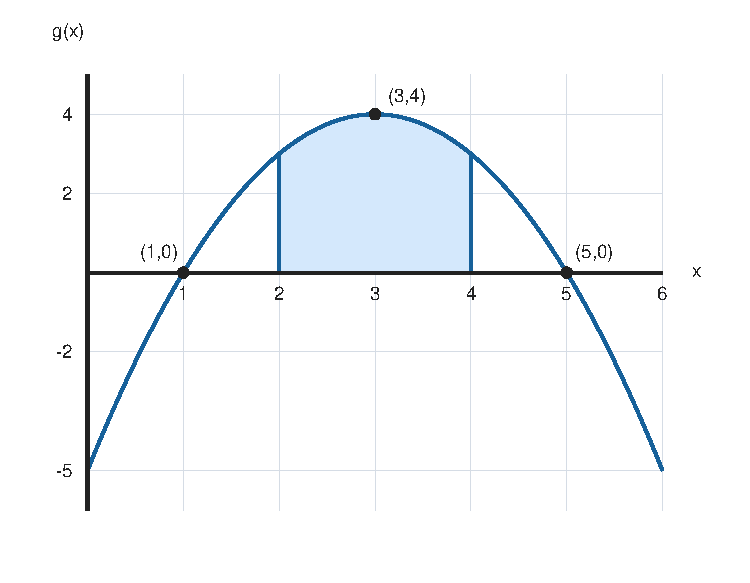
\includegraphics[width=0.57\linewidth]{recursos/figuras/s015-area.pdf}\end{center}
\[
\begin{aligned}
\mathcal A&=\int_2^4(-x^2+6x-5)\,dx\\
&=\left[-\frac{x^3}{3}+3x^2-5x\right]_2^4
=\frac{20}{3}-\left(-\frac23\right)=\boxed{\frac{22}{3}\text{ unidades cuadradas}.}
\end{aligned}
\]
También se obtiene con $u=x-3$: $\int_{-1}^1(4-u^2)\,du=8-2/3=22/3$.
